\chapter{Existing Approaches in Behavior Analysis and Detection of Customer Satisfaction}
\label{ch:backgroundResearch}
As the cornerstones of the research objectives have been defined, the goal is to shed more light onto the key point this thesis deals with, namely Customer Satisfaction. The following chapter defines the term Customer Satisfaction and outlines which properties are paid attention to in this thesis. Moreover, existing approaches related to analysis of usage behavior and measurement of Customer Satisfaction, with focus on their relevance regarding this thesis, will be discussed in more detail.

\section{Definition and Limitations of Customer Satisfaction interpretation}
\label{sec:custSatisfactionDefinition}
Before evluating approaches to determine Customer Satisfaction via collected knowledge data, the term should be properly understood. Impactful research papers regarding the definition of Customer Satisfaction were already published in the 70s. Since then different approaches viewing the topic from slightly different angles have been proposed. A popular statement, namely that Customer Satisfaction is based on the comparison between individual expectations of the customer and the perceived performance of the product after usage was the common result of research experiments at these times \cite{oliver1977effect} \cite{anderson1973consumer}. If his or her expectations were lower or equal, the customer can be considered as satisfied whereas vice versa the customer is dissatisfied since his expectations were not fulfilled. In case the expectations do not match with the actual performance of the product this is also named positive- respectively negative disconfirmation while a match is described as confirmation \cite{oliver1977effect} \cite{anderson1973consumer}.

As a result, when imagining it in a more mathematical way Customer Satisfaction can be represented as a simple function with two input parameters. One the one hand, the expectations of the customer are based on all information gathered before using the product. It is an subjectively built ideal picture of the product depending on advertisement, word-of-mouth critics and company- respectively brand reputation \cite{johnson2001evolution} \cite{neckel2015}. On the other hand the perceived performance of the product when using it comprises the whole consumption experience of the customer. As the main driver of this experience, the overall provided quality of the product was identified. This perceived quality metric not only covers the pure quality, in terms or whether the product reliably performs as advertised, but more exactly specifies the actual quality for the price. Thus, when talking about drivers of Customer Satisfaction it is often described as perceived value \cite{johnson2001evolution} \cite{fornell1992national}. Along with the shift towards importance of customer retention, Customer Satisfaction models developed from a transaction tied view to a cumulative view which considers a customers experience with a product over a longer time period. This view more specifically includes the fact that customer expectations change over time and become influential for the perceived quality as well. \cite{johnson1996expectations}. It became clear that the Customer Satisfaction construct is quite involved and especially some of the antecedents and consequenes remained unclear. 

The Swedish Customer Satisfaction Barometer (SCSB) was a big research project in investigating Customer Satisfaction across several industries within a whole country. It used a model based on the two identified input parameters from previous research. The positive result of Customer Satisfaction was already anticipated by \cite{bolton1998dynamic} \cite{gustafsson2005effects}. The outcome of dissatisfaction was based on the theory of \cite{hulett1971exit} that customers are more likely to complain for problems they might have. Furthermore the model stated that postive resolving of complaints supports the establishment of loyalty against the company. A sketch of this model is shown in figure \ref{fig:scsb}

\begin{figure}
	\centering
	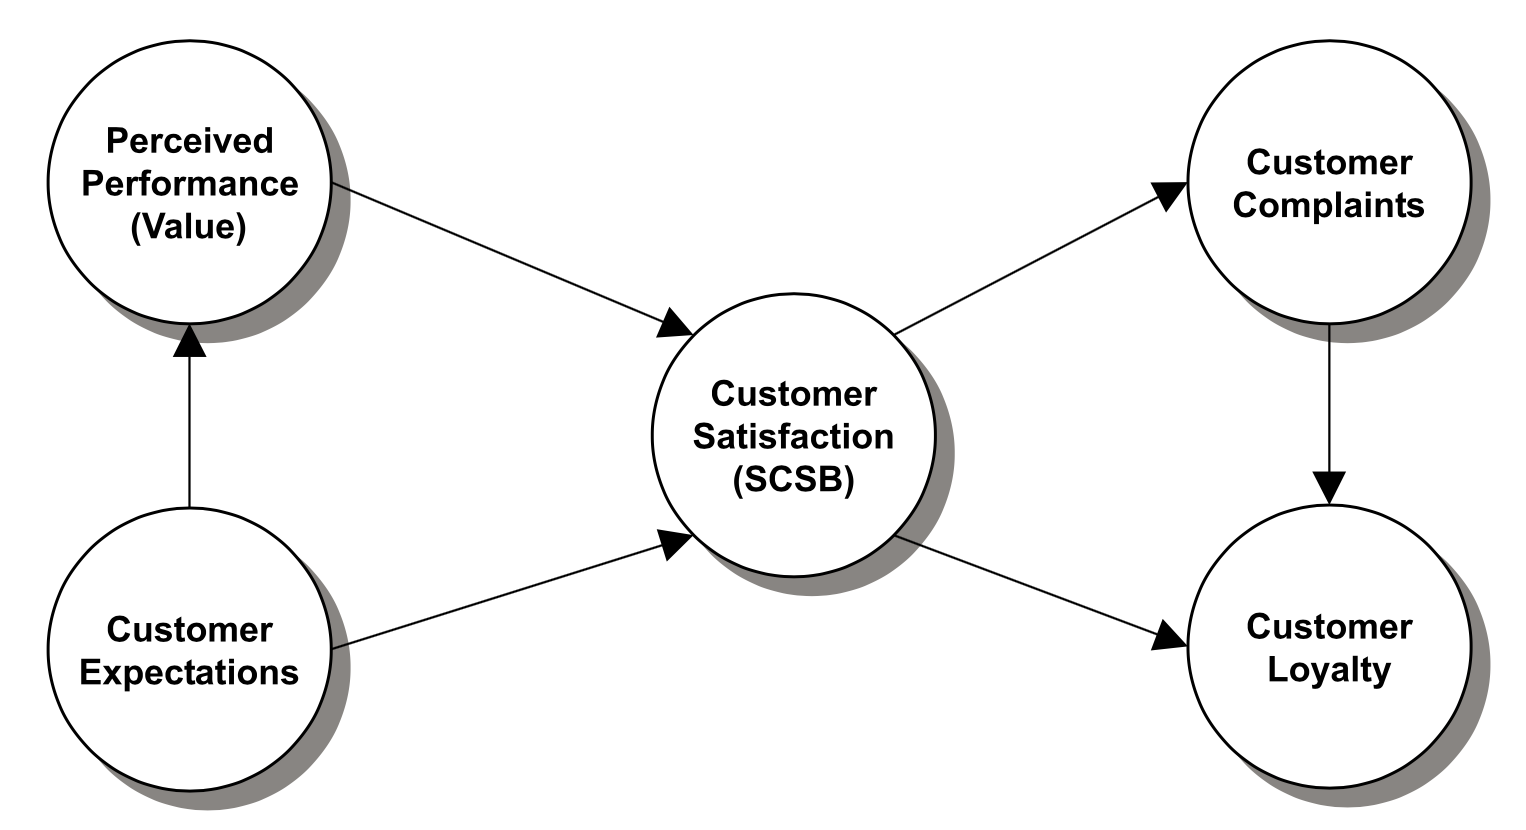
\includegraphics[width=1.0\textwidth]{img/scsb.png}
	\caption{Model used for Swedish Customer Satisfaction barometer\cite{fornell1992national}}
	\label{fig:scsb}
\end{figure} 

Although the model experienced some critics in the following years as further national Customer Satisfaction surveys were deployed they all were based on and inspired by the original ideas of the swedish model. A more enhanced analysis of the existing model approaches was done by \cite{johnson2001evolution}. As a result of the derived strengths and weaknesses from different Customer Satisfaction barometer models, they proposed a new model which will be used as the base model by this thesis to build its further empirical work on. The model is visualized in figure \ref{fig:satisfactionModel}. Each of the different parts will be described briefly to get an overview on the essential components and their relationships, adaptions in contrast to the initial base model, namely the SCSB, and the limitations drawn by the author regarding the work in this thesis. 

\begin{figure}
	\centering
	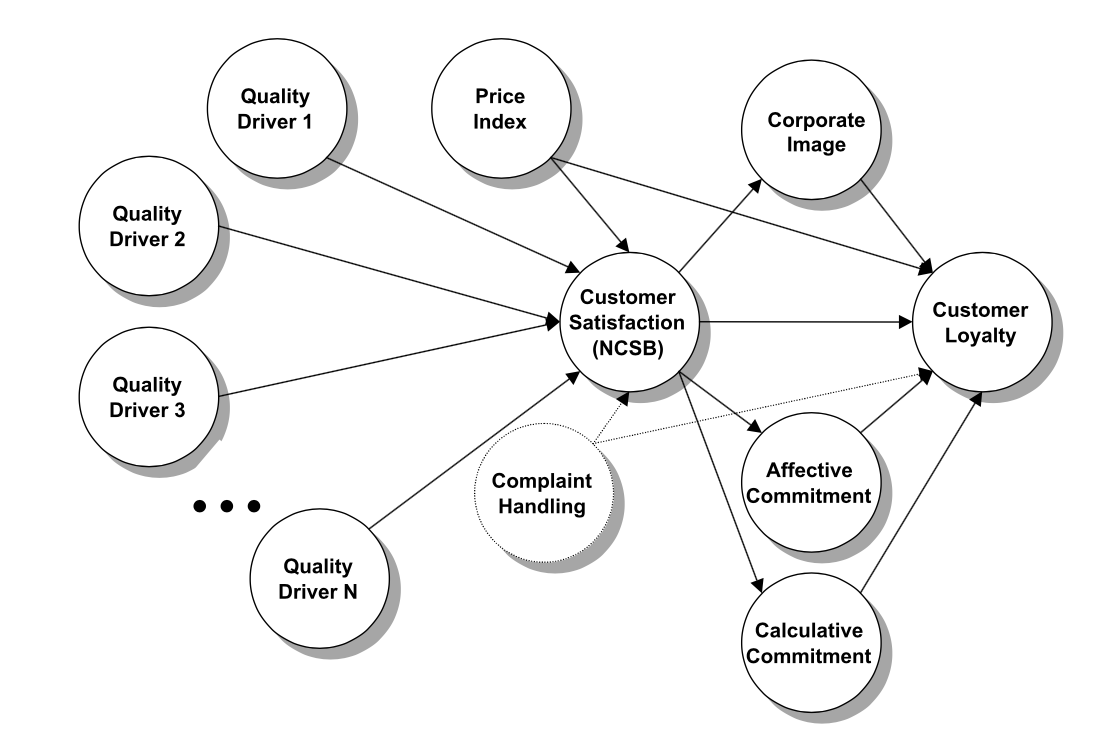
\includegraphics[width=1.0\textwidth]{img/custSatisfaction.png}
	\caption{Customer satisfaction model proposed by \cite{johnson2001evolution}}
	\label{fig:satisfactionModel}
\end{figure} 

The first clear difference when comparing the latter proposed model with the SCSB is the role of customer expectations. Since satisfaction has to be observed within a long time period, expectations get adapted throughout repeated consumption experience as well. More emphasis is put on the quality delivered by the product and the expectations are considered to be evaluated regularly due this quality. These statements can be supported among several industries including thet communications sector which the author considers as similar to the sector the case study of this thesis operates in \cite{johnson1996expectations} \cite{fornell1996american}. Despite that fact the author does not completely agree with these findings to remove the term "customer expecations" totally. Instead of the expectation parameter, 1-n perceived quality criterion are predictors for Customer Satisfaction. Next to the quality drivers the perceived price for the provided product quality plays a role as well. The third satisfaction driver illustrated in this model are complaint handling. Due to evolvement of customer support services, customer complaints cannot be stated as simple negative outcome of Customer Satisfaction. More specifically customer care influences emotions either negatively or positively and as a consequence is in direct predictor relationship to satisfaction. It may even have an impact on repurchase behavior of customers which explains the direct relationship to customer loyalty \cite{johnson2001evolution}. 

The three remaining components have not yet been mentioned explicity regarding their role in the customer satisfaction construct. All of them are directly influenced by the outcome of Customer Satisfaction while mediating the loyalty parameter. The corporate image, or sometimes called brand reputation, indicates how popular and known company is in the public. Consumption experiences of a customer affects the corporate image in a certain direction as well. According to a study of \cite{hussain2015service} a dissatisfied customer tells on average nine other people about negative experiences which can heavily affect loyalty. Although the coporate image is part of the model it will not be discussed or used further in the empirical work of this thesis because it can not be measured by usage behavior and quality data. Similarly the affective- and calculative commitment mediate parts of the effect of Customer Satisfaction on customer loyalty. While the affective component resides on the emotional side and mainly relates to trust with regard to a brand, the calculative component is more rational in terms of costs. (e.g.: costs for a customer to cancel a relationship and switcht to a competitor) \cite{johnson2001evolution} Both components were mentioned for the purpose of completness but are not elaborated in more detail since they cannot be represented in the available data of the case study. 

\section{Measurement of Customer Satisfaction}
As the reader got an overview on the parts and influencers of Customer Satisfaction, the next step is to look at possiblities to transform the defined model properties to quantiative measurements. On the one hand this thesis evaluated survey based measurements and looked in more detail on different types and their performance. On the other hand it was tried to find approaches to measure Customer Satisfaction without survey data based on implicit satisfaction representing patterns in huge data sets. 

Although there has been a lot of research regarding a formal definition of Customer Satisfaction, less papers were published on how this satisfaction can be quantitatively measured. One approach based on the original expectancy-performance disconfirmation model was to design a survey asking customers how they would rate

\begin{itemize}
	\item the perceived performance and quality of the product with regard to a set of chosen dimension of the product and
	\item their expectations regarding the same set of dimension before the usage \cite{prakash1983reliability}.
\end{itemize}

This approach seems to be promising as it respects the originally identfied and well researched Customer Satisfaction model. However, it brings problems with it and thus make it inappropriate for this thesis. Firstly, expectations can hardly be measured unbiased since they get evaluated by the customer alongside with the perceived quality in case of using one satisfaction survey \cite{getty1995relationship}. As outlined in \ref{custSatisfactionDefinition} the proposed model is based on cumulative satisfaction evaluation which yield regular adaptions on what a customer expect from a product. Asking customers about their expectations, with regard to a specific set of product dimensions, explicitly before usage neither makes any sense from a business prespective of Tractive nor is the author able to initiate a process to collect such data. Secondly, measuring customer expectations turns out to be difficult in general as people tend to rate their expectations, if they have to state them explicitly, very high in general \cite{babakus1992empirical}. As a consequence the uniform overrating of customers expectations will not provide any extra information in assessing customer satisfaction from a survey.


The beginning of research work in terms of measuring and analyzing how satisfied users are with a computer system already dates back to the beginning of the 80s. At these times first researchers supposed that there is a relationship between user satisfaction and the success of a computer system. From this point on, a series of researches investigated which factors could influence user satisfaction and how to ask users to get a representative opinion \cite{roy1998developing}. Bailey \& Pearson were first to propose a questionnaire consisting of 39 satisfaction dimensions which should help information system providers to evaluate whether a user is satisfied with the system or not. Ives, Olsen \& Baroudi did some further research based on the existing work from Bailey \& Pearson to reduce the effort for users to answer 39 dimensions. However technology changed dramatically as the shift towards the use of personal computers started a few years later and therefore new approaches were needed. According to Doll and Torkzadeh the previous developed methods did not focus on the satisfaction with a specific end-user application since they do not cover the human-machine interaction \cite{roy1998developing}. Thus, they developed a model specifying the end-user satisfaction as a second factor driven by five first-order factors namely content, format, accuracy, timeliness and ease of use. After testing four different models regarding validity and reliability using a confirmatory factor analysis approach against some sample data, they came up with the following model visualized in figure ~\ref{fig:relatedDoll}. 

\begin{figure}
	\centering
	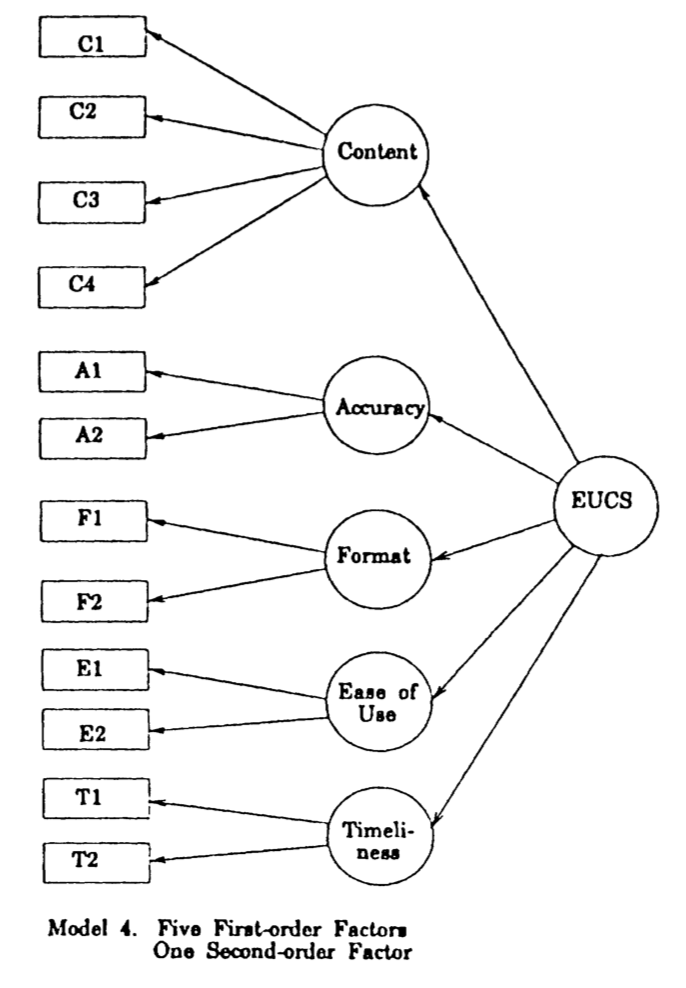
\includegraphics[width=1.0\textwidth]{img/dollSecondFactor.png}
	\caption{Customer Satisfaction - Five first-order factors \cite{doll1994confirmatory}}
	\label{fig:relatedDoll}
\end{figure} 

In the results for this model they claim that 74\% of the variation in the five first-order factors is explained by the end-user satisfaction. \cite{doll1994confirmatory}. This second-factor approach turned out to be quite successful over the following years and has been widely used to reason about user satisfaction for specific applications. The web has been evolving rapidly and due to this reason \cite{xiao2002measurement} analyzed in their research in 2002 whether the existing method of Doll and Torkzadeh is still appropriate and applicable to web-based information systems. They recognized that some of the previously identified factors may not be relevant anymore for web-based information systems. Based on the work of Doll and Torkzadeh, a questionnaire was created to ask people how satisfied they are with a web based information system whereby they decided to choose Internet Portals as representative example. The results of this research showed that the existing five factors are still valid under these new circumstances. However, the research clearly has some limitations as it only considered Internet Portals and did not look on additional factors like privacy or security \cite{xiao2002measurement}. In 1999 \cite{roy1998developing} took a closer look on several existing measurement approaches and discussed their limitations in practice. In contrast to \cite{xiao2002measurement} the results of this research tend to be more critical regarding practical usefulness of approaches like the one from Doll and Torkzadeh. They criticize that surveyed users are considered with equal personality and behavior whereas in practice each individual user is different and this would therefore require an independent consideration in a survey. Furthermore the research claims that existing survey approaches are often too inflexible since a service provider has specific objectives and the survey has to put more focus on certain aspects than others which cannot be achieved without modifications. Meanwhile researchers recognized that besides extracting knowledge about customer satisfaction explicitly, there is another promising opportunity to implicitly understand behavior of customers based on how they present themselves, act and behave. Supported by the rapid growth of software technology and tools the era of statistical analysis and data mining in CRM started up in the beginning of the 21st century \cite{Ngai2009} \cite{neckel2015}. The research paper of \cite{Ngai2009} wrapped up CRM quite comprehensively by taking a closer look onto 87 selected published journals dealing with CRM and Data Mining techniques. They tried to find out how the distribution of publications among the different areas of CRM looks like and as a result came to the conclusion that statistical and data mining techniques are especially in customer retention of great interest. A promising approach reasoning about dissatisfaction of customers and its connection to churn was proposed by \cite{mozer2000predicting}. This research project first of all analyzed influencing factors driving customers in the wireless telecommunications industry to stay or leave the service. After identifying major factors differentiating between satisfied and dissatisfied customers, statistical machine learning techniques as logistic regression, decision trees and neural networks were employed to predict churn rate for a selected time period. Later on \cite{mozer2000predicting} outlines a calculation model to determine under which circumstances it makes sense to offer an incentive to a potential churner and take the opportunity to pursue him/her to stay. Based on the variables of lost revenue due to a churner, acquisition costs of a new customer, the probability of staying after offered an incentive and the cost of offering an incentive to a customer, an cost saving per customer could be calculated. The results clearly showed that in most cases taking the effort of offering incentives and thus preventing churn results in higher profitability. Due to the similarity, considering the recurring payment service type as well as properties and nature of competition on the market, with the illustration example outlined in~\ref{sec:illustrationExample}, the research of \cite{mozer2000predicting} supports the practical work conveyed by this thesis. Another related research work published by \cite{lariviere2005predicting} dealt with analysis of customer behavior and its impact on retention and profitability for a European Financial Institute. Using a data set of about 100k customers and advanced decision tree algorithm, namely Random Forest, was employed to perform a binary classification based on the properties of whether a customer

\begin{itemize}
	\item buys a further banking product in the future,
	\item cancels a non-ending relationship with a purchased product,
	\item or causes a profit drop within a considered time period.
\end{itemize}

In a further stage the Random Forest algorithm was also used to analyze which of the identified independent variables affect the outcome factors related to customer retention remarkably. As surprising side effect it was found out that some of the variables show an influencing effect in all three binary classifiers although they seem quite contrary as the new-buy and cancellation of a product for instance. 

The previous work from \cite{mozer2000predicting} and \cite{lariviere2005predicting} already shows the power of statistical and machine learning techniques to predict future customer behavior and its effect on retention and profitability. It was clearly indicated that past customer behavior data turns out to be worthy in recognizing patterns, relationships and predicting the future. Since customer satisfaction is usually a rather complex construct consisting of several dimensions besides purchase, cancellation and profit evolution of a product, there is enough potential to reveal hidden patterns and answer business critical questions regarding customers behavior. Moreover statistical tools and data mining techniques have evolved further and demand for a reappraisal. According to \cite{gantz2012digital} only half a percent of the data available in the digital universe is analyzed but in 2020 about 33\% of all data may be valuable which supports the assumption that there is still a lot of work ahead. 




